\chapter{Design and Implementation}

\section{System Architecture}

The proposed system is designed based on a Centralized Barrier synchronization model \cite{PaDSS}, where a central entity, referred to as the \textbf{Simulation Executive}, coordinates the synchronization and communication among all other processes in the simulation. Each process interacts with the Simulation Executive to communicate its state and synchronize its progress. When all processes have communicated their current state, the Simulation Executive determines the minimum simulation time that all processes can safely advance to, ensuring consistent progression.

This centralized approach reduces the overall communication overhead significantly. In a typical client-server simulation with $m$ client requests, the number of synchronization messages can reach $O(nm)$, where $n$ is the number of processes, and each request results in at least one `syncSleep(T)` call. Our architecture optimizes this to achieve $O(m)$ synchronization messages by eliminating redundant broadcasts to all processes and instead notifying only the process with the lowest simulation time. The overall system architecture is depicted in Figure~\ref{fig:arch}.

\begin{figure}[H]
    \centering
    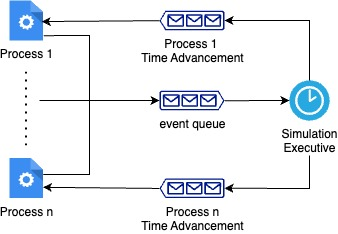
\includegraphics[width=0.7\textwidth]{images/architecture_program.jpg}
    \caption{System Architecture}
    \label{fig:arch}
\end{figure}

Although this approach introduces additional complexity in managing the state of each process, it significantly reduces the number of messages transmitted over the network, leading to an overall performance improvement. At the start of the simulation, each process establishes a connection with the Simulation Executive, creating a dedicated messaging stream. The Simulation Executive handles all connections and disconnections dynamically, ensuring seamless communication and synchronization.

\section{Component Design}

The implementation of the Simulation Executive requires careful consideration of several key components and mechanisms:

\begin{itemize}
    \item \textbf{Event List Management}: Efficient management of the event list is crucial to handle scheduling operations effectively. We employ a priority queue \cite{pqueue} to manage events, allowing insertion and removal of the minimum element in $O(\log n)$ time, where $n$ is the number of events.

    \item \textbf{Managing Simulation Time Advances}: The Simulation Executive must correctly manage the states of all connected processes and handle various edge cases. The simulation time can advance if and only if:

    \begin{center}
        \#\text{list\_management} \\ = \\  n - \#\text{disconnected\_processes} - \#\text{processes\_in\_blocking\_call}
    \end{center}

    This formula ensures that the simulation time advances only when all active processes are ready. Each process in the system can exist in one of the following states:

    \begin{itemize}
        \item \textbf{Running}: The process is actively executing instructions.
        \item \textbf{Sleeping}: The process is waiting in the event list.
        \item \textbf{Blocking}: The process is waiting for a message or response.
        \item \textbf{Disconnected}: The process has left the simulation and is no longer participating.
    \end{itemize}

    To manage these states efficiently, we use an unordered map \cite{umap}, which supports $O(1)$ operations for insertion, deletion, and element counting.
\end{itemize}

\section{Process Interaction Primitives}

The interaction between the processes and the Simulation Executive is facilitated through a set of primitive functions:

\begin{itemize}
    \item \textbf{connect()}: Establishes a connection between a process and the Simulation Executive.
    \item \textbf{alertBlockingCall()}: Notifies the Simulation Executive that the process is waiting for a message or response.
    \item \textbf{exitBlockingCall()}: Notifies the Simulation Executive that the process has exited the blocking state.
    \item \textbf{syncSleep(long double T)}: Signals that the process will resume after a specified simulated time \( T \).
    \item \textbf{mySleep(long double T)}: Emulates real-time sleep, allowing the process to pause for \( T \) time units.
    \item \textbf{disconnect()}: Disconnects the process from the Simulation Executive.
\end{itemize}

Using these primitives, we define the behavior of client, server, and service processes in the simulation. The pseudocode for each process is presented below:

\begin{algorithm}[H]
\caption{Client Behavior Simulation} \label{alg:client_simulation}
\begin{algorithmic}[1]
    \STATE \textbf{Initialize} client parameters.
    \WHILE{True}
        \STATE mySleep(based on the current state)
        \STATE syncSleep(time to send a request)
        \STATE Send a request corresponding to the current state.
        \STATE alertBlockingCall()
        \STATE Wait for the server's response.
        \STATE exitBlockingCall()
        \STATE syncSleep(time to update the state)
        \STATE Update state: $state \leftarrow newState(state)$
    \ENDWHILE
\end{algorithmic}
\end{algorithm}

\begin{algorithm}[H]
\caption{Server Request Handling} \label{alg:server_request_handling}
\begin{algorithmic}[1]
    \STATE \textbf{Initialize} server parameters.
    \WHILE{True}
        \STATE alertBlockingCall()
        \STATE Wait for incoming requests from clients or services.
        \STATE exitBlockingCall()
        \STATE syncSleep(time to process the request)
        \IF{the request is from a client}
            \STATE Forward the request to the corresponding service.
        \ELSE
            \STATE Send the response back to the client.
        \ENDIF
    \ENDWHILE
\end{algorithmic}
\end{algorithm}

\begin{algorithm}[H]
\caption{Service Response Handling} \label{alg:service_response_handling}
\begin{algorithmic}[1]
    \STATE \textbf{Initialize} service parameters.
    \WHILE{True}
        \STATE alertBlockingCall()
        \STATE Wait for requests from the server.
        \STATE exitBlockingCall()
        \STATE syncSleep(time to process the request)
        \STATE Send the response back to the server.
    \ENDWHILE
\end{algorithmic}
\end{algorithm}

\section{Managing Synchronization Issues}

One of the primary challenges in implementing a centralized synchronization model is handling delays caused by network latency. Figure~\ref{fig:IssueImp} illustrates potential synchronization issues when processes transition between different states.

\begin{figure}[H]
    \centering
    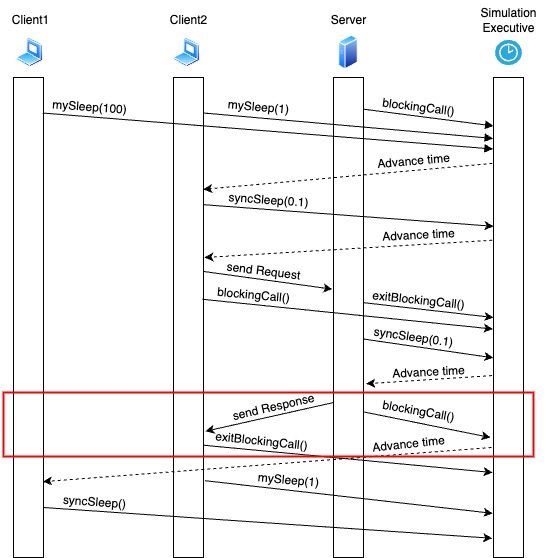
\includegraphics[width=1\linewidth]{images/IssueImp.jpg}
    \caption{Space-Time Diagram of the Simulation}
    \label{fig:IssueImp}
\end{figure}

For instance, after sending a request, `client1` might enter a `Sleeping` state, while `client2` is in a `Blocking` state, waiting for a response from the server. To address these issues, we introduce an additional state:

\begin{itemize}
    \item \textbf{Ready to Exit Blocking Call}: Represents processes that are in a blocking state but are expected to receive a response shortly.
\end{itemize}

To support this state, we define the following additional primitives:

\begin{itemize}
    \item \textbf{sendId(std::string id)}: Associates each process with a unique identifier, facilitating easier tracking of communications.
    \item \textbf{sendingTo(std::string receiverId)}: Notifies the Simulation Executive that a process is sending a message to `receiverId`, allowing it to anticipate a blocking exit.
\end{itemize}

The updated condition for simulation time advancement now becomes:

\begin{center}
    \#\text{list\_management} \\ = \\  n - \#\text{disconnected\_processes} - (\#\text{processes\_in\_blocking\_call} - \#\text{processes\_exiting\_blocking\_call})
\end{center}

This refinement ensures that simulation time advances correctly even under varying network conditions and communication delays.

\subsection*{Simulation Executive}

To start the Simulation Executive, specify the number of processes expected to connect. The executive will then wait for connections to be established with each process before initiating the simulation.

\subsection*{Simulation Application}

The system includes default classes such as `Client`, `Server`, and `Service`, which ensure correct interaction with the Simulation Executive. Custom processes can also be implemented using the described primitives to interact seamlessly with the Simulation Executive, allowing for flexible simulation scenarios, there are also a provided classes that simulate the client based on some inputs, server, and services.


\section{Monitoring and Logging Mechanism}

The system includes two critical components for tracking simulation activities and collecting performance metrics: the \textbf{Simulation Logger} and the \textbf{Performance Monitor}. These components are designed to provide real-time insights into the simulation, detect anomalies, and enable efficient debugging. Such a monitoring architecture follows principles similar to distributed logging systems, which enhance observability and fault detection by aggregating data from multiple sources, thereby offering a comprehensive view of system performance \cite{MediumDistributedLogging}. Figure~\ref{fig:monitors} depicts an illustration of these monitoring mechanisms.

\begin{figure}[H]
    \centering
    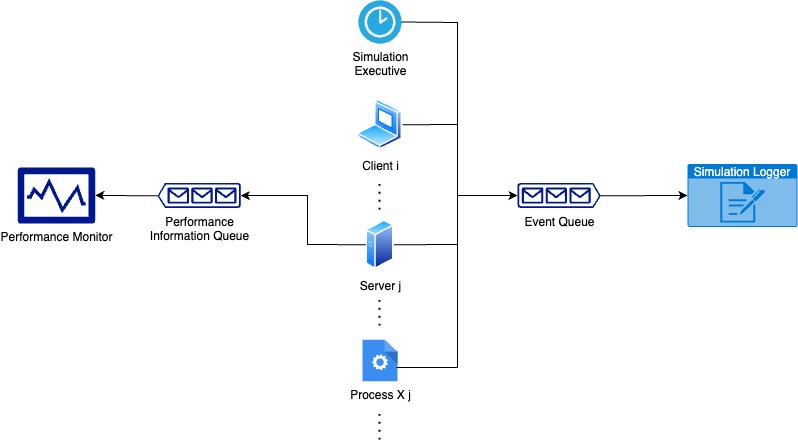
\includegraphics[width=0.7\textwidth]{images/monitors.jpg}
    \caption{Monitoring and Logging Mechanism}
    \label{fig:monitors}
\end{figure}

\subsection{Simulation Logger}

The \textbf{Simulation Logger} records all significant events that occur during the simulation. Each event is logged with the following details:

\begin{itemize}
    \item \textbf{Timestamp}: The timestamp when the event occurred.
    \item \textbf{Event Type}: The type of event (e.g., `connection established`, `alertBlockingCall`, etc.).
    \item \textbf{Stream Name}: The stream where the event originated.
    \item \textbf{Values}: Any associated data relevant to the event.
\end{itemize}

This detailed logging allows for comprehensive post-simulation analysis, facilitating the identification of execution patterns, interactions between processes, and debugging of unexpected behavior.

\subsection{Performance Monitor}

The \textbf{Performance Monitor} collects and analyzes performance metrics during the simulation. It continuously receives data from connected servers and updates key statistics such as:

\begin{itemize}
    \item \textbf{Average Response Time}: The mean response time for all processed requests.
    \item \textbf{Minimum Response Time}: The shortest observed response time.
    \item \textbf{Maximum Response Time}: The longest observed response time.
    \item \textbf{Variance}: The variance in response times, which indicates the consistency of the system's performance.
\end{itemize}

The Performance Monitor not only identifies and alerts users of potential bottlenecks but also allows them to intervene during the simulation. This proactive capability helps in addressing performance issues as they emerge, minimizing disruptions. All performance logs are stored for post-simulation analysis, enabling a comprehensive evaluation of the system's efficiency and facilitating more granular analysis, such as tracing specific inefficiencies or assessing particular scenarios that might have led to performance degradation.

